% !TeX program = lualatex
\documentclass[11pt,a4paper]{article}
\usepackage{fontspec}
\setmainfont{DejaVu Sans}
\usepackage{babel}\babelprovide[main,import]{lithuanian}
\usepackage{amsmath,amssymb,tikz,array,geometry,tcolorbox,fancyhdr}
\usetikzlibrary{angles,quotes,calc,arrows.meta}
\geometry{left=17mm,right=17mm,top=15mm,bottom=16mm,headheight=14pt}
\definecolor{ink}{HTML}{183249}\definecolor{blue}{HTML}{176A96}\definecolor{gold}{HTML}{CD7610}\definecolor{soft}{HTML}{EDF5F9}
\pagestyle{fancy}\fancyhf{}\fancyfoot[L]{\small\color{ink} Bazinės geometrijos sąvokos, žymėjimai, susitarimai}\fancyfoot[R]{\small\thepage}\renewcommand{\headrulewidth}{0pt}\renewcommand{\footrulewidth}{0pt}
\setlength{\parindent}{0pt}\setlength{\parskip}{4pt}
\newcommand{\headpage}[2]{\noindent{\small\bfseries\color{blue} Bazinės geometrijos sąvokos, žymėjimai, susitarimai}\par\vspace{2mm}{\LARGE\bfseries\color{ink}#1}\par\vspace{1mm}{\small\color{ink}#2}\par\vspace{3mm}}
\newcommand{\boxrow}[3]{\begin{tcolorbox}[colback=white,colframe=blue!43,boxrule=.45pt,arc=2mm,left=3mm,right=3mm,top=2mm,bottom=2mm]\noindent\begin{minipage}[c]{.32\linewidth}\centering #2\end{minipage}\hfill\begin{minipage}[c]{.64\linewidth}\raggedright\textbf{\color{ink}#1}\par\vspace{1mm}#3\end{minipage}\end{tcolorbox}\vspace{1mm}}
\newcommand{\note}[1]{\begin{tcolorbox}[colback=soft,colframe=blue!40,arc=2mm,boxrule=.4pt,left=3mm,right=3mm,top=2mm,bottom=2mm]\raggedright #1\end{tcolorbox}}
\newcommand{\dotp}[3]{\fill (#1,#2) circle (1.6pt) node[#3] {$#3$};}
\begin{document}
\headpage{Taškas, tiesė, atkarpa ir spindulys}{Andrius Berniukevičius · Vilniaus licėjus}
\note{Čia pateikiamos pagrindinės geometrijos sąvokos, jų žymėjimai ir pagrindinės savybės. Taškas ir tiesė yra \textbf{pradinės sąvokos}: jų neapibrėžiame kitomis sąvokomis, tik paaiškiname vaizdžiai.}
\boxrow{Taškas}{
\begin{tikzpicture}\fill[blue](0,0) circle (2pt) node[above right]{$A$};\end{tikzpicture}}{Taškas nurodo vietą plokštumoje. Jį žymime didžiąja raide, pavyzdžiui, $A$. Brėžinyje tašką vaizduojame mažu taškeliu.}
\boxrow{Tiesė}{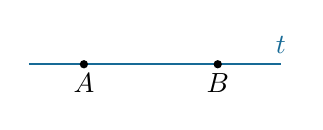
\begin{tikzpicture}[>=Latex]\draw[blue,thick](-.2,0)--(3,0) node[above]{$t$};\fill (.5,0) circle(1.5pt) node[below]{$A$};\fill (2.2,0) circle(1.5pt) node[below]{$B$};\end{tikzpicture}}{Tiesė be galo tęsiasi į abi puses. Ją žymime mažąja raide, pavyzdžiui, $t$, arba dviejų skirtingų jos taškų raidėmis: tiesė $AB$. Užrašas $A\in t$ reiškia, kad taškas $A$ priklauso tiesei $t$.}
\boxrow{Atkarpa}{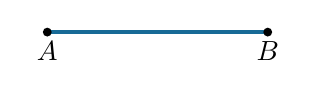
\begin{tikzpicture}\draw[blue,very thick](0,0)--(2.8,0);\fill (0,0) circle(1.6pt) node[below]{$A$};\fill (2.8,0) circle(1.6pt) node[below]{$B$};\end{tikzpicture}}{Atkarpa $AB$ sudaryta iš taškų $A$, $B$ ir visų tarp jų esančių tiesės $AB$ taškų. Taškai $A,B$ – jos galai. Žymuo $AB$ pagal kontekstą taip pat reiškia atkarpos ilgį; pavyzdžiui, $AB=4\text{ cm}$.}
\boxrow{Spindulys}{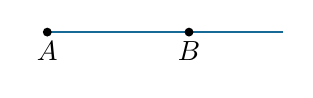
\begin{tikzpicture}[>=Latex]\draw[blue,thick](0,0)--(3,0);\fill (0,0) circle(1.6pt) node[below]{$A$};\fill (1.8,0) circle(1.6pt) node[below]{$B$};\end{tikzpicture}}{Spindulys $AB$ prasideda taške $A$, eina per $B$ ir tęsiasi ta pačia kryptimi. $A$ yra jo pradžios taškas. Priešingi spinduliai turi bendrą pradžią ir sudaro tiesę.}
\note{\textbf{Pagrindinės savybės.} Per du skirtingus taškus eina tik viena tiesė. Jei taškas $C$ yra tarp taškų $A$ ir $B$, tai $AC+CB=AB$. Lygindami atkarpų ilgius, juos išreiškiame tais pačiais matavimo vienetais.}
\newpage
\headpage{Kampai}{Kampų žymėjimas, matavimas ir rūšys.}
\boxrow{Kampas ir jo žymėjimas}{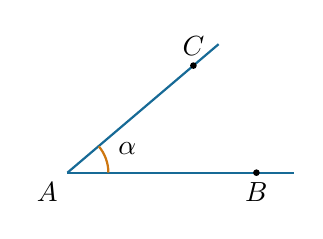
\begin{tikzpicture}[scale=.8,>=Latex]\coordinate(A)at(0,0);\coordinate(B)at(3,0);\coordinate(C)at(2,1.7);\draw[blue,thick](A)--($(A)!1.2!(B)$);\draw[blue,thick](A)--($(A)!1.2!(C)$);\fill (B) circle(1.5pt);\fill (C) circle(1.5pt);\draw[gold,thick](.65,0) arc(0:40:.65);\node[below left]at(A){$A$};\node[below]at(B){$B$};\node[above]at(C){$C$};\node at(.95,.38){$\alpha$};\end{tikzpicture}}{Du skirtingi iš vieno taško išeinantys spinduliai sudaro kampo kraštines; bendras jų pradžios taškas yra \textbf{viršūnė}. $\angle BAC$ viršūnė yra $A$. Kampus arba jų dydžius žymime ir graikiškomis raidėmis:\par $\alpha$ – tariame \textbf{alfa}, $\beta$ – \textbf{beta},\par $\gamma$ – \textbf{gama}, $\theta$ – \textbf{teta}.}
\begin{tcolorbox}[colback=white,colframe=blue!43,arc=2mm,boxrule=.45pt]\textbf{\color{ink}Kampų rūšys}\par\vspace{2mm}
\centering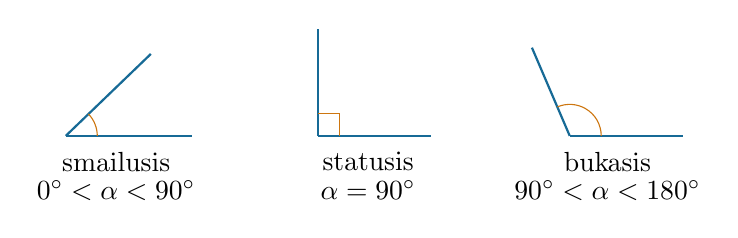
\begin{tikzpicture}[scale=.8,>=Latex]
\begin{scope}[shift={(0,0)}]\draw[blue,thick](0,0)--(2,0);\draw[blue,thick](0,0)--(1.35,1.3);\draw[gold](.5,0)arc(0:44:.5);\node[below]at(.8,-.1){smailusis};\node[below]at(.8,-.55){$0^\circ<\alpha<90^\circ$};\end{scope}
\begin{scope}[shift={(4,0)}]\draw[blue,thick](0,0)--(1.8,0);\draw[blue,thick](0,0)--(0,1.7);\draw[gold](.35,0)--(.35,.35)--(0,.35);\node[below]at(.8,-.1){statusis};\node[below]at(.8,-.55){$\alpha=90^\circ$};\end{scope}
\begin{scope}[shift={(8,0)}]\draw[blue,thick](0,0)--(1.8,0);\draw[blue,thick](0,0)--(-.6,1.4);\draw[gold](.5,0)arc(0:113:.5);\node[below]at(.6,-.1){bukasis};\node[below]at(.6,-.55){$90^\circ<\alpha<180^\circ$};\end{scope}
\end{tikzpicture}\par\vspace{2mm}\raggedright\textbf{Ištiestinis kampas}: jo kraštinės yra spinduliai, esantys vienoje tiesėje, o dydis – $180^\circ$.\quad 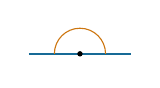
\begin{tikzpicture}[baseline=-.5ex,scale=.65,>=Latex]\draw[blue,thick](-1,0)--(1,0);\fill(0,0)circle(1.5pt);\draw[gold](.5,0)arc(0:180:.5);\end{tikzpicture}
\end{tcolorbox}
\boxrow{Kampo pusiaukampinė}{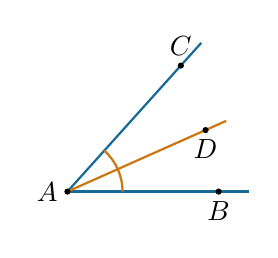
\begin{tikzpicture}[scale=.8,>=Latex]\coordinate(A)at(0,0);\coordinate(B)at(2.4,0);\coordinate(C)at(1.8,2);\coordinate(D)at(24.006:2.4);\draw[blue,thick](A)--($(A)!1.2!(B)$);\draw[blue,thick](A)--($(A)!1.18!(C)$);\draw[gold,thick](A)--($(A)!1.15!(D)$);\foreach \p/\pos in {A/left,B/below,C/above,D/below}{\fill(\p)circle(1.4pt)node[\pos]{$\p$};}\pic[draw=gold,thick,angle radius=7mm] {angle=B--A--D};\pic[draw=gold,thick,angle radius=7mm] {angle=D--A--C};\end{tikzpicture}}{Kampo $BAC$ pusiaukampinė – iš viršūnės $A$ išeinantis spindulys $AD$, dalijantis šį kampą į du lygius kampus: $\angle BAD=\angle DAC$.}
\note{\textbf{Kampų matavimas.} Kampų dydžius matuojame laipsniais. Jei spindulys $AD$ eina kampo $BAC$ viduje, tai $\angle BAD+\angle DAC=\angle BAC$.}
\newpage
\headpage{Gretutiniai ir kryžminiai kampai, priekampis}{Šių kampų savybes taikome spręsdami geometrijos uždavinius.}
\boxrow{Gretutiniai kampai}{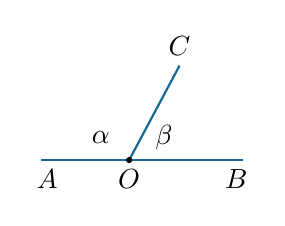
\begin{tikzpicture}[scale=.8,>=Latex]\draw[blue,thick](-1.4,0)--(1.8,0);\draw[blue,thick](0,0)--(.8,1.5);\fill(0,0)circle(1.4pt)node[below]{$O$};\node[below]at(-1.3,0){$A$};\node[below]at(1.7,0){$B$};\node[above]at(.8,1.5){$C$};\node at(-.45,.35){$\alpha$};\node at(.55,.35){$\beta$};\end{tikzpicture}}{Du kampai vadinami gretutiniais, jei turi bendrą kraštinę, o kitos jų kraštinės yra priešingi spinduliai. Gretutinių kampų suma lygi $180^\circ$:\par $\alpha+\beta=180^\circ$.}
\boxrow{Kryžminiai kampai}{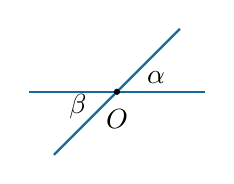
\begin{tikzpicture}[scale=.8,>=Latex]\draw[blue,thick](-1.4,0)--(1.4,0);\draw[blue,thick](-1,-1)--(1,1);\fill(0,0)circle(1.4pt)node[below=3pt]{$O$};\node at(.62,.23){$\alpha$};\node at(-.62,-.23){$\beta$};\end{tikzpicture}}{Du kampai vadinami \textbf{kryžminiais}, jei vieno kampo kraštinės yra kito kampo kraštinių priešingi spinduliai. Tokie kampai susidaro susikertant dviem tiesėms. Kryžminiai kampai yra lygūs: $\alpha=\beta$.}
\boxrow{Trikampio priekampis}{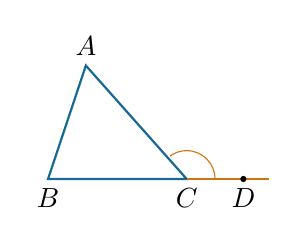
\begin{tikzpicture}[scale=.8,>=Latex]\coordinate(A)at(.6,1.8);\coordinate(B)at(0,0);\coordinate(C)at(2.2,0);\coordinate(D)at(3.1,0);\draw[blue,thick](A)--(B)--(C)--cycle;\draw[gold,thick](C)--($(C)!1.45!(D)$);\fill (D) circle (1.4pt);\node[above]at(A){$A$};\node[below]at(B){$B$};\node[below]at(C){$C$};\node[below]at(D){$D$};\draw[gold](2.65,0)arc(0:126:.45);\end{tikzpicture}}{Pratęsus trikampio kraštinę $BC$ už viršūnės $C$, kampas $ACD$ vadinamas trikampio \textbf{priekampiu} ties viršūne $C$. Jis gretutinis vidaus kampui $ACB$, todėl jų suma lygi $180^\circ$.}
\note{\textbf{Kaip skaityti brėžinį?} Brėžinys padeda suprasti, kurie taškai, atkarpos ir spinduliai nagrinėjami. Tačiau vien iš vaizdo negalime spręsti, kad atkarpos yra lygios ar statmenos: tai turi būti nurodyta uždavinio sąlygoje arba pažymėta brėžinyje.}
\newpage
\headpage{Trikampis ir jo žymėjimai}{Sutarti žymėjimai padeda suprasti uždavinių sąlygas ir įrodymus.}
\boxrow{Trikampis}{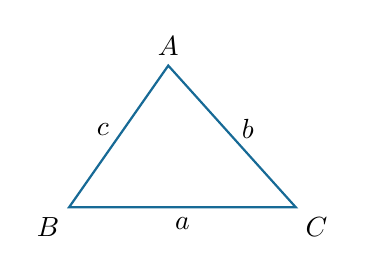
\begin{tikzpicture}[scale=.9]\coordinate(A)at(1.4,2);\coordinate(B)at(0,0);\coordinate(C)at(3.2,0);\draw[blue,thick](A)--(B)--(C)--cycle;\node[above]at(A){$A$};\node[below left]at(B){$B$};\node[below right]at(C){$C$};\node[below]at(1.6,0){$a$};\node[right]at(2.3,1.1){$b$};\node[left]at(.7,1.1){$c$};\end{tikzpicture}}{Trikampį $ABC$ sudaro trys vienoje tiesėje nesantys taškai $A,B,C$ ir juos jungiančios atkarpos. Prieš kiekvieną viršūnę esančios kraštinės ilgį žymime atitinkama mažąja raide:\par $a=BC$, $b=CA$, $c=AB$.}
\boxrow{Lygiašonis trikampis}{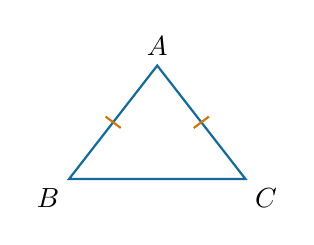
\begin{tikzpicture}[scale=.8]\coordinate(A)at(1.4,1.8);\coordinate(B)at(0,0);\coordinate(C)at(2.8,0);\draw[blue,thick](A)--(B)--(C)--cycle;\draw[gold,thick] ($(B)!.5!(A)+(-.12,.09)$)--($(B)!.5!(A)+(.12,-.09)$) ($(C)!.5!(A)+(-.12,-.09)$)--($(C)!.5!(A)+(.12,.09)$);\node[above]at(A){$A$};\node[below left]at(B){$B$};\node[below right]at(C){$C$};\end{tikzpicture}}{Lygiašonis trikampis turi bent dvi lygias kraštines. Jei $AB=AC$, tai $BC$ vadinama pagrindu, o $AB$ ir $AC$ – šoninėmis kraštinėmis. Lygias kraštines žymime vienodais brūkšneliais.}
\boxrow{Lygiakraštis trikampis}{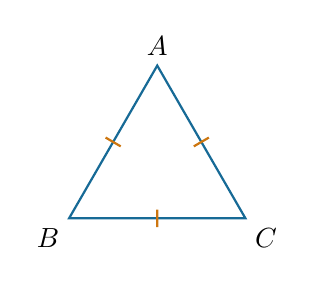
\begin{tikzpicture}[scale=.8]\coordinate(A)at(1.4,2.42487);\coordinate(B)at(0,0);\coordinate(C)at(2.8,0);\draw[blue,thick](A)--(B)--(C)--cycle;\draw[gold,thick] ($(B)!.5!(A)+(-.12,.07)$)--($(B)!.5!(A)+(.12,-.07)$) ($(C)!.5!(A)+(-.12,-.07)$)--($(C)!.5!(A)+(.12,.07)$) (1.4,-.14)--(1.4,.14);\node[above]at(A){$A$};\node[below left]at(B){$B$};\node[below right]at(C){$C$};\end{tikzpicture}}{Lygiakraštis trikampis turi tris lygias kraštines: $AB=BC=CA$. Todėl pagal pasirinktą apibrėžimą jis taip pat yra lygiašonis. Įvairiakraščio trikampio visų trijų kraštinių ilgiai skirtingi.}
\boxrow{Vidurio taškas}{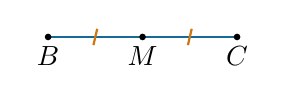
\begin{tikzpicture}[scale=.8]\draw[blue,thick](0,0)--(3,0);\foreach \x/\lab in {0/B,1.5/M,3/C}{\fill(\x,0)circle(1.5pt)node[below]{$\lab$};}\draw[gold,thick](.72,-.13)--(.78,.13) (2.22,-.13)--(2.28,.13);\end{tikzpicture}}{Taškas $M$ yra atkarpos $BC$ vidurio taškas, jei taškas $M$ priklauso atkarpai $BC$ ir $BM=MC$. Vienodais brūkšneliais pažymėtos atkarpos laikomos lygiomis.}
\note{\textbf{Žymėjimo susitarimai.} Kraštines ir jų ilgius žymime $a,b,c$. Kai reikia pažymėti kelis panašiai apibrėžtus taškus, rašome indeksus, pavyzdžiui, $M_a,M_b,M_c$ arba $M_1,M_2,M_3$. Ką reiškia indeksas, nurodome sąlygoje arba paaiškiname prie brėžinio.}
\newpage
\headpage{Trikampių rūšys pagal kampus}{Trikampius skirstome į smailiuosius, stačiuosius ir bukuosius.}
\boxrow{Smailusis trikampis}{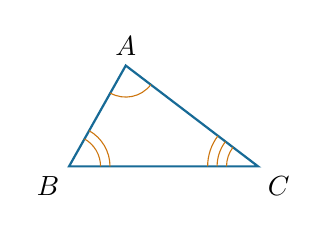
\begin{tikzpicture}[scale=.8]\coordinate(A)at(.9,1.6);\coordinate(B)at(0,0);\coordinate(C)at(3,0);\draw[blue,thick](A)--(B)--(C)--cycle;\pic[draw=gold,angle radius=4mm] {angle=B--A--C};\foreach \r in {4,5.2}{\pic[draw=gold,angle radius=\r mm] {angle=C--B--A};}\foreach \r in {4,5.2,6.4}{\pic[draw=gold,angle radius=\r mm] {angle=A--C--B};}\node[above]at(A){$A$};\node[below left]at(B){$B$};\node[below right]at(C){$C$};\end{tikzpicture}}{Smailusis trikampis – trikampis, kurio visi trys kampai yra smailieji, t.~y. mažesni už $90^\circ$.}
\boxrow{Statusis trikampis}{\begin{tikzpicture}[scale=.8]\coordinate(A)at(0,2);\coordinate(B)at(0,0);\coordinate(C)at(2.8,0);\draw[blue,thick](A)--(B)node[midway,left]{statinis}--(C)node[midway,below]{statinis}--cycle;\path(A)--(C)node[midway,above,sloped]{įžambinė};\draw[gold](.25,0)--(.25,.25)--(0,.25);\node[above]at(A){$A$};\node[below left]at(B){$B$};\node[below right]at(C){$C$};\end{tikzpicture}}{Statusis trikampis – trikampis, kurio vienas kampas yra statusis, t.~y. lygus $90^\circ$. Statųjį kampą sudarančios kraštinės vadinamos \textbf{statiniais}, o prieš statųjį kampą esanti kraštinė – \textbf{įžambine}. Brėžinyje statiniai yra $AB$ ir $BC$, įžambinė – $AC$.}
\boxrow{Bukasis trikampis}{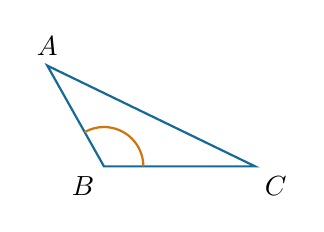
\begin{tikzpicture}[scale=.8]\coordinate(A)at(-.9,1.6);\coordinate(B)at(0,0);\coordinate(C)at(2.4,0);\draw[blue,thick](A)--(B)--(C)--cycle;\pic[draw=gold,thick,angle radius=5mm] {angle=C--B--A};\node[above]at(A){$A$};\node[below left]at(B){$B$};\node[below right]at(C){$C$};\end{tikzpicture}}{Bukasis trikampis – trikampis, kurio vienas kampas yra bukasis, t.~y. didesnis už $90^\circ$, bet mažesnis už $180^\circ$. Brėžinyje bukasis kampas yra $\angle ABC$.}
\note{\textbf{Du skirstymo būdai.} Trikampius skirstome pagal kraštinių ilgius ir pagal kampų dydžius. Tas pats trikampis gali būti, pavyzdžiui, ir lygiašonis, ir statusis.}
\newpage
\headpage{Pusiaukraštinė, aukštinė, pusiaukampinė}{Šių atkarpų apibrėžimai ir jų ilgių žymėjimas.}
\boxrow{Pusiaukraštinė $m_a$}{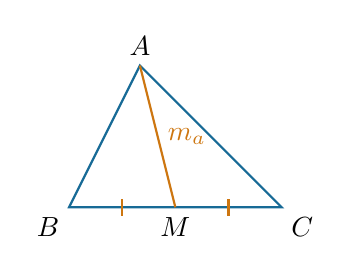
\begin{tikzpicture}[scale=.9]\coordinate(A)at(1,2);\coordinate(B)at(0,0);\coordinate(C)at(3,0);\coordinate(M)at(1.5,0);\draw[blue,thick](A)--(B)--(C)--cycle;\draw[gold,thick](A)--(M)node[midway,right]{$m_a$};\draw[gold,thick](.75,-.12)--(.75,.12) (2.25,-.12)--(2.25,.12);\node[above]at(A){$A$};\node[below left]at(B){$B$};\node[below right]at(C){$C$};\node[below]at(M){$M$};\end{tikzpicture}}{Trikampio pusiaukraštinė – atkarpa, jungianti viršūnę su priešingos kraštinės vidurio tašku. Jei $BM=MC$, tai $AM$ yra pusiaukraštinė į kraštinę $a=BC$. Jos ilgį žymime $m_a=AM$.}
\boxrow{Aukštinė $h_a$}{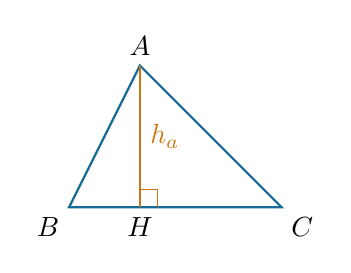
\begin{tikzpicture}[scale=.9]\coordinate(A)at(1,2);\coordinate(B)at(0,0);\coordinate(C)at(3,0);\coordinate(H)at(1,0);\draw[blue,thick](A)--(B)--(C)--cycle;\draw[gold,thick](A)--(H)node[midway,right]{$h_a$};\draw[gold](1.25,0)--(1.25,.25)--(1,.25);\node[above]at(A){$A$};\node[below left]at(B){$B$};\node[below right]at(C){$C$};\node[below]at(H){$H$};\end{tikzpicture}}{Aukštinė – atkarpa, nubrėžta iš viršūnės statmenai (sudarant $90^\circ$ kampą) tiesei, kurioje yra priešinga kraštinė. $H$ yra statmens pagrindas, $AH\perp BC$, o $h_a=AH$. Aukštinės pagrindas gali būti ir už pačios kraštinės ribų.}
\boxrow{Aukštinė bukajame trikampyje}{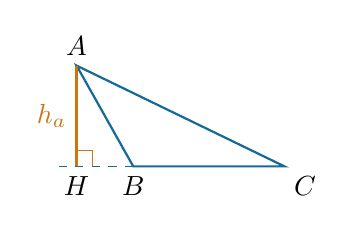
\begin{tikzpicture}[scale=.8]\coordinate(A)at(-.9,1.6);\coordinate(B)at(0,0);\coordinate(C)at(2.4,0);\coordinate(H)at(-.9,0);\draw[blue,thick](A)--(B)--(C)--cycle;\draw[blue,dashed](B)--(-1.2,0);\draw[gold,thick](A)--(H)node[midway,left]{$h_a$};\draw[gold](-.65,0)--(-.65,.25)--(-.9,.25);\node[above]at(A){$A$};\node[below]at(B){$B$};\node[below right]at(C){$C$};\node[below]at(H){$H$};\end{tikzpicture}}{Trikampio $ABC$ kampas $ABC$ yra bukasis. Iš viršūnės $A$ nubrėžtos aukštinės $AH$ pagrindas $H$ yra kraštinės $BC$ tęsinyje už viršūnės $B$. Kraštinės tęsinys pažymėtas brūkšnine linija. Kaip ir anksčiau, $AH\perp BC$, o $h_a=AH$.}
\boxrow{Pusiaukampinė $l_a$}{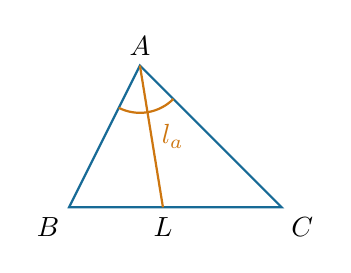
\begin{tikzpicture}[scale=.9]\coordinate(A)at(1,2);\coordinate(B)at(0,0);\coordinate(C)at(3,0);\coordinate(L)at(1.325,0);\draw[blue,thick](A)--(B)--(C)--cycle;\draw[gold,thick](A)--(L)node[midway,right]{$l_a$};\pic[draw=gold,thick,angle radius=6mm] {angle=B--A--L};\pic[draw=gold,thick,angle radius=6mm] {angle=L--A--C};\node[above]at(A){$A$};\node[below left]at(B){$B$};\node[below right]at(C){$C$};\node[below]at(L){$L$};\end{tikzpicture}}{Trikampio pusiaukampinė – kampo pusiaukampinės atkarpa nuo viršūnės iki priešingos kraštinės. Ji dalija trikampio kampą į du lygius kampus. Jei $\angle BAL=\angle LAC$, tai $AL$ – pusiaukampinė, o jos ilgis $l_a=AL$.}
\note{\textbf{Žymėjimo susitarimai.} Raidėmis $m_a,h_a,l_a$ žymime atitinkamų atkarpų \emph{ilgius}. Trumpumo dėlei sakome ir „pusiaukraštinė $m_a$“. Kitų kraštinių vidurio taškus žymime $M_b,M_c$, aukštinių pagrindus – $H_b,H_c$, o pusiaukampinių ir priešingų kraštinių susikirtimo taškus – $L_b,L_c$. Prireikus vartojame ir skaitinius indeksus.}
\newpage
\headpage{Tiesių tarpusavio padėtys}{Statmenumas, lygiagretumas ir lygiagretumo prielaida.}
\boxrow{Statmenos tiesės}{\begin{tikzpicture}[scale=.8,>=Latex]\draw[blue,thick](-1.5,0)--(1.5,0)node[right]{$p$};\draw[blue,thick](0,-.9)--(0,1.3)node[above]{$q$};\draw[gold](.3,0)--(.3,.3)--(0,.3);\end{tikzpicture}}{Dvi tiesės yra statmenos, jei jos susikirsdamos sudaro statųjį kampą. Žymime $p\perp q$. Atstumas nuo taško iki tiesės – iš to taško į tiesę nubrėžto statmens ilgis.}
\boxrow{Atkarpos vidurio statmuo}{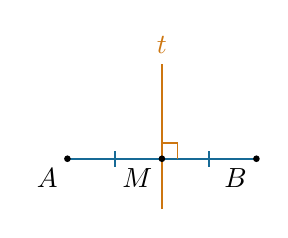
\begin{tikzpicture}[scale=.8]\coordinate(A)at(0,0);\coordinate(B)at(3,0);\coordinate(M)at(1.5,0);\draw[blue,thick](A)--(B);\draw[gold,thick](1.5,-.8)--(1.5,1.5)node[above]{$t$};\draw[gold](1.75,0)--(1.75,.25)--(1.5,.25);\draw[blue,thick](.75,-.13)--(.75,.13) (2.25,-.13)--(2.25,.13);\foreach \p in {A,B,M}{\fill(\p)circle(1.5pt)node[below left]{$\p$};}\end{tikzpicture}}{Atkarpos \textbf{vidurio statmuo} – tiesė, einanti per atkarpos vidurio tašką ir statmena tai atkarpai. Brėžinyje $AM=MB$ ir $t\perp AB$. Skirtingai nuo trikampio aukštinės, vidurio statmuo yra tiesė ir nebūtinai eina per trikampio viršūnę.}
\boxrow{Lygiagrečiosios tiesės}{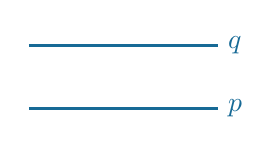
\begin{tikzpicture}[scale=.8,>=Latex]\draw[blue,thick](-1.5,0)--(1.5,0)node[right]{$p$};\draw[blue,thick](-1.5,1)--(1.5,1)node[right]{$q$};\end{tikzpicture}}{Dvi \textbf{skirtingos} vienoje plokštumoje esančios tiesės yra lygiagrečiosios, jei jos nesikerta. Žymime $p\parallel q$.}
\boxrow{Lygiagretumo prielaida}{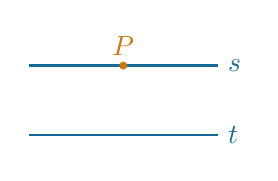
\begin{tikzpicture}[scale=.8]\draw[blue,thick](-1.5,0)--(1.5,0)node[right]{$t$};\draw[blue,thick](-1.5,1.1)--(1.5,1.1)node[right]{$s$};\fill[gold](0,1.1)circle(1.8pt)node[above]{$P$};\end{tikzpicture}}{Plokštumą įsivaizduokime kaip neribotą plokščią paviršių. Jei taškas $P$ nėra tiesėje $t$, per $P$ eina \textbf{tik viena} tiesė $s$, lygiagreti $t$. Šį faktą Euklido geometrijoje priimame kaip pradinę prielaidą.}
\newpage
\headpage{Iškilieji ir neiškilieji keturkampiai}{Juos skiriame pagal įstrižainių padėtį arba vidaus kampų dydžius.}
\boxrow{Keturkampis ir įstrižainės}{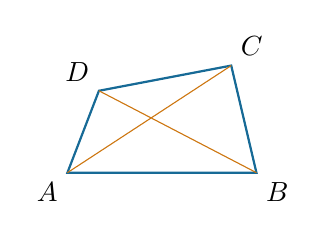
\begin{tikzpicture}[scale=.8]\coordinate(A)at(0,0);\coordinate(B)at(3,0);\coordinate(C)at(2.6,1.7);\coordinate(D)at(.5,1.3);\draw[blue,thick](A)--(B)--(C)--(D)--cycle;\draw[gold](A)--(C) (B)--(D);\node[below left]at(A){$A$};\node[below right]at(B){$B$};\node[above right]at(C){$C$};\node[above left]at(D){$D$};\end{tikzpicture}}{Keturkampį $ABCD$ sudaro keturios nuoseklios kraštinės $AB,BC,CD,DA$ ir jų apribota sritis. Kraštinės nesikerta, išskyrus gretimų kraštinių bendrus galus; jokios trys viršūnės nėra vienoje tiesėje. Atkarpos $AC$ ir $BD$, jungiančios negretimas viršūnes, yra \textbf{įstrižainės}.}
\boxrow{Iškilasis keturkampis}{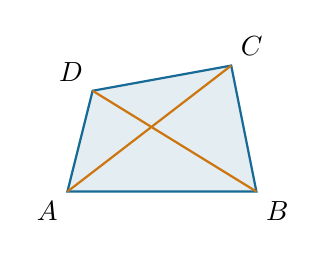
\begin{tikzpicture}[scale=.8]\coordinate(A)at(0,0);\coordinate(B)at(3,0);\coordinate(C)at(2.6,2);\coordinate(D)at(.4,1.6);\fill[blue!12](A)--(B)--(C)--(D)--cycle;\draw[blue,thick](A)--(B)--(C)--(D)--cycle;\draw[gold,thick](A)--(C) (B)--(D);\node[below left]at(A){$A$};\node[below right]at(B){$B$};\node[above right]at(C){$C$};\node[above left]at(D){$D$};\end{tikzpicture}}{Keturkampis vadinamas \textbf{iškiluoju}, jei visi jo vidaus kampai yra mažesni už $180^\circ$. Abi jo įstrižainės, išskyrus jų galus, yra keturkampio viduje.}
\boxrow{Neiškilasis keturkampis}{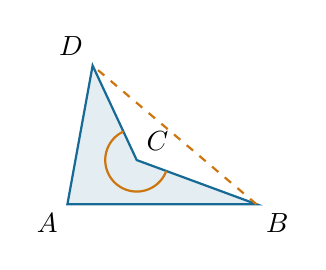
\begin{tikzpicture}[scale=.8]\coordinate(A)at(0,0);\coordinate(B)at(3,0);\coordinate(C)at(1.1,.7);\coordinate(D)at(.4,2.2);\fill[blue!12](A)--(B)--(C)--(D)--cycle;\draw[blue,thick](A)--(B)--(C)--(D)--cycle;\draw[gold,thick,dashed](B)--(D);\pic[draw=gold,thick,angle radius=4mm] {angle=D--C--B};\node[below left]at(A){$A$};\node[below right]at(B){$B$};\node[above right]at(C){$C$};\node[above left]at(D){$D$};\end{tikzpicture}}{Keturkampis vadinamas \textbf{neiškiluoju}, jei viena jo įstrižainė, išskyrus galus, yra už keturkampio ribų. Brėžinyje tai įstrižainė $BD$, pažymėta brūkšnine linija. Tą patį galima nusakyti ir kampu: vienas vidaus kampas yra didesnis už $180^\circ$. Brėžinyje lankeliu pažymėtas toks kampas ties viršūne $C$.}
\boxrow{Perimetras}{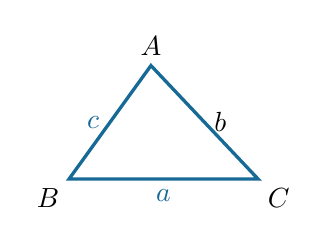
\begin{tikzpicture}[scale=.8]\coordinate(A)at(1.3,1.8);\coordinate(B)at(0,0);\coordinate(C)at(3,0);\draw[blue,very thick](A)--(B)node[midway,left]{$c$}--(C)node[midway,below]{$a$}--cycle;\path(A)--(C)node[midway,right]{$b$};\node[above]at(A){$A$};\node[below left]at(B){$B$};\node[below right]at(C){$C$};\end{tikzpicture}}{Daugiakampio \textbf{perimetras} – visų jo kraštinių ilgių suma. Perimetrą žymime raide $P$. Trikampio perimetras $P=a+b+c$, o keturkampio $ABCD$ perimetras $P=AB+BC+CD+DA$. Visus ilgius išreiškiame tais pačiais matavimo vienetais.}
\newpage
\headpage{Keturkampių rūšys}{Trapecija, lygiagretainis, stačiakampis, rombas ir kvadratas.}
\boxrow{Trapecija}{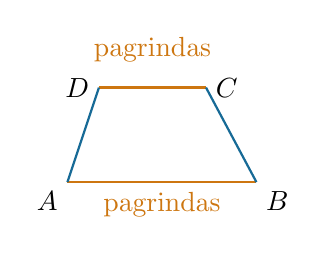
\begin{tikzpicture}[scale=.8]\coordinate(A)at(0,0);\coordinate(B)at(3,0);\coordinate(C)at(2.2,1.5);\coordinate(D)at(.5,1.5);\draw[gold,thick](A)--(B)node[midway,below]{pagrindas} (D)--(C)node[midway,above=2mm]{pagrindas};\draw[blue,thick](A)--(D) (B)--(C);\node[below left]at(A){$A$};\node[below right]at(B){$B$};\node[right]at(C){$C$};\node[left]at(D){$D$};\end{tikzpicture}}{Trapecija – keturkampis, kurio \textbf{tik viena} priešingųjų kraštinių pora yra lygiagreti. Brėžinyje $AB\parallel CD$. Šios kraštinės vadinamos \textbf{pagrindais}, kitos dvi, $AD$ ir $BC$, – \textbf{šoninėmis kraštinėmis}. Pagal šį apibrėžimą lygiagretainis nėra trapecija.}
\boxrow{Lygiagretainis}{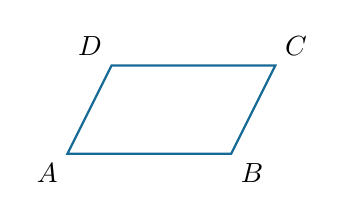
\begin{tikzpicture}[scale=.8]\coordinate(A)at(0,0);\coordinate(B)at(2.6,0);\coordinate(C)at(3.3,1.4);\coordinate(D)at(.7,1.4);\draw[blue,thick](A)--(B)--(C)--(D)--cycle;\node[below left]at(A){$A$};\node[below right]at(B){$B$};\node[above right]at(C){$C$};\node[above left]at(D){$D$};\end{tikzpicture}}{Lygiagretainis – keturkampis, kurio abi priešingųjų kraštinių poros yra lygiagrečios: $AB\parallel DC$ ir $AD\parallel BC$.}
\boxrow{Stačiakampis}{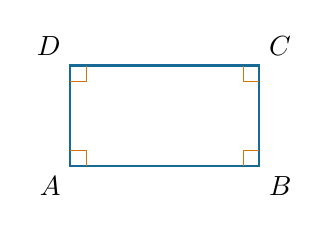
\begin{tikzpicture}[scale=.8]\coordinate(A)at(0,0);\coordinate(B)at(3,0);\coordinate(C)at(3,1.6);\coordinate(D)at(0,1.6);\draw[blue,thick](A)--(B)--(C)--(D)--cycle;\draw[gold](.25,0)--(.25,.25)--(0,.25) (2.75,0)--(2.75,.25)--(3,.25) (3,1.35)--(2.75,1.35)--(2.75,1.6) (.25,1.6)--(.25,1.35)--(0,1.35);\node[below left]at(A){$A$};\node[below right]at(B){$B$};\node[above right]at(C){$C$};\node[above left]at(D){$D$};\end{tikzpicture}}{Stačiakampis – keturkampis, kurio visi keturi kampai yra statieji, t.~y. lygūs $90^\circ$. Jis taip pat yra lygiagretainis.}
\boxrow{Rombas}{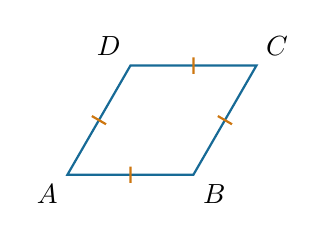
\begin{tikzpicture}[scale=.8]\coordinate(A)at(0,0);\coordinate(B)at(2,0);\coordinate(C)at(3,1.73205);\coordinate(D)at(1,1.73205);\draw[blue,thick](A)--(B)--(C)--(D)--cycle;\draw[gold,thick](1,-.13)--(1,.13) (2,1.60205)--(2,1.86205) (2.3874,.93103)--(2.6126,.80103) (.3874,.93103)--(.6126,.80103);\node[below left]at(A){$A$};\node[below right]at(B){$B$};\node[above right]at(C){$C$};\node[above left]at(D){$D$};\end{tikzpicture}}{Rombas – keturkampis, kurio visos keturios kraštinės yra lygios: $AB=BC=CD=DA$. Jis taip pat yra lygiagretainis.}
\boxrow{Kvadratas}{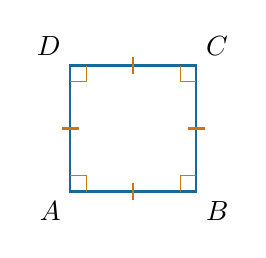
\begin{tikzpicture}[scale=.8]\coordinate(A)at(0,0);\coordinate(B)at(2,0);\coordinate(C)at(2,2);\coordinate(D)at(0,2);\draw[blue,thick](A)--(B)--(C)--(D)--cycle;\draw[gold](.25,0)--(.25,.25)--(0,.25) (1.75,0)--(1.75,.25)--(2,.25) (2,1.75)--(1.75,1.75)--(1.75,2) (.25,2)--(.25,1.75)--(0,1.75);\draw[gold,thick](1,-.13)--(1,.13) (1,1.87)--(1,2.13) (-.13,1)--(.13,1) (1.87,1)--(2.13,1);\node[below left]at(A){$A$};\node[below right]at(B){$B$};\node[above right]at(C){$C$};\node[above left]at(D){$D$};\end{tikzpicture}}{Kvadratas – keturkampis, kurio visos keturios kraštinės yra lygios ir visi keturi kampai yra statieji. Kvadratas yra ir stačiakampis, ir rombas, todėl taip pat yra lygiagretainis.}
\newpage
\headpage{Apskritimas ir skritulys}{Atstumas nuo centro leidžia apibrėžti abi figūras.}
\boxrow{Apskritimas}{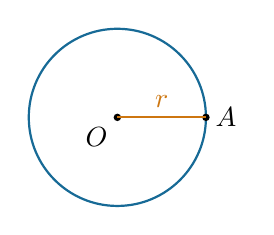
\begin{tikzpicture}[scale=.9]\draw[blue,thick](0,0)circle(1.25);\fill(0,0)circle(1.5pt)node[below left]{$O$};\fill(1.25,0)circle(1.5pt)node[right]{$A$};\draw[gold,thick](0,0)--(1.25,0)node[midway,above]{$r$};\end{tikzpicture}}{Apskritimas – figūra, sudaryta iš visų plokštumos taškų, nuo taško $O$ nutolusių tuo pačiu atstumu $r>0$. $O$ – \textbf{centras}, $r$ – \textbf{spindulio ilgis}. Taškas $A$ yra apskritime tada ir tik tada, kai $OA=r$.}
\boxrow{Skritulys}{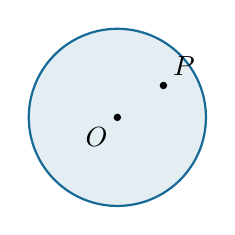
\begin{tikzpicture}[scale=.9]\fill[blue!12](0,0)circle(1.25);\draw[blue,thick](0,0)circle(1.25);\fill(0,0)circle(1.5pt)node[below left]{$O$};\fill(.65,.45)circle(1.5pt)node[above right]{$P$};\end{tikzpicture}}{Skritulys – figūra, sudaryta iš visų plokštumos taškų, kurių atstumas nuo centro $O$ yra ne didesnis kaip $r$. Taigi $P$ priklauso skrituliui, jei $OP\le r$. Apskritimas yra skritulio riba.}
\boxrow{Spindulys, styga, skersmuo}{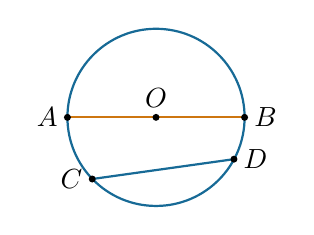
\begin{tikzpicture}[scale=.9]\draw[blue,thick](0,0)circle(1.25);\draw[gold,thick](-1.25,0)--(1.25,0);\draw[blue,thick](-.9,-.87)--(1.1,-.59);\fill(0,0)circle(1.4pt)node[above]{$O$};\fill(-1.25,0)circle(1.4pt)node[left]{$A$};\fill(1.25,0)circle(1.4pt)node[right]{$B$};\fill(-.9,-.87)circle(1.4pt)node[left]{$C$};\fill(1.1,-.59)circle(1.4pt)node[right]{$D$};\end{tikzpicture}}{Atkarpa $OA$ yra \textbf{spindulys}. Atkarpa $CD$, jungianti du apskritimo taškus, yra \textbf{styga}. Per centrą einanti styga $AB$ yra \textbf{skersmuo}. Skersmens ilgis yra dvigubai didesnis už spindulio ilgį: $AB=2r$.}
\boxrow{Tiesė ir apskritimas}{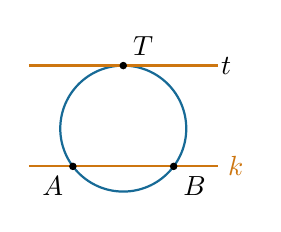
\begin{tikzpicture}[scale=.8,>=Latex]\draw[blue,thick](0,0)circle(1);\draw[gold,thick](-1.5,1)--(1.5,1);\fill(0,1)circle(1.7pt)node[above right]{$T$};\node[right]at(1.4,1){$t$};\draw[gold,thick](-1.5,-.6)--(1.5,-.6)node[right]{$k$};\fill(-.8,-.6)circle(1.7pt)node[below left]{$A$};\fill(.8,-.6)circle(1.7pt)node[below right]{$B$};\end{tikzpicture}}{Tiesė, su apskritimu turinti vieną bendrą tašką, vadinama \textbf{liestine}, o tas taškas $T$ – lietimosi tašku. Tiesė, kertanti apskritimą dviejuose taškuose, vadinama \textbf{kirstine}. Brėžinyje $t$ yra liestinė, o $k$ – kirstinė, kertanti apskritimą taškuose $A$ ir $B$.}
\newpage
\headpage{Du trikampių lygumo požymiai}{Šiuos požymius taikome norėdami nustatyti, ar trikampiai lygūs.}
\note{\textbf{Trikampių lygumas.} Trikampiai yra lygūs, jei vieną galima uždėti ant kito taip, kad jie sutaptų. Užrašas $\triangle ABC = \triangle DEF$ nurodo ir atitinkamas viršūnes: $A\leftrightarrow D$, $B\leftrightarrow E$, $C\leftrightarrow F$. Taikant lygumo požymį, nebūtina atskirai palyginti visų kraštinių ir kampų.}
\boxrow{Pagal dvi kraštines ir kampą tarp jų}{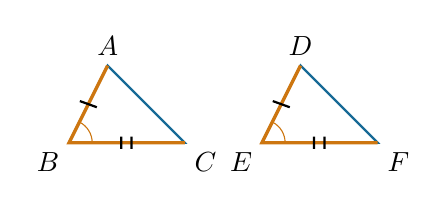
\begin{tikzpicture}[scale=.49]\foreach \shift/\A/\B/\C in {0/A/B/C,5/D/E/F}{\begin{scope}[xshift=\shift cm]\draw[blue,thick](0,0)--(3,0)--(1,2)--cycle;\draw[gold,very thick](1,2)--(0,0)--(3,0);\draw[black,thick](.28,1.08)--(.72,.92) (1.35,-.16)--(1.35,.16) (1.62,-.16)--(1.62,.16);\draw[gold](.6,0)arc(0:63:.6);\node[above]at(1,2){$\A$};\node[below left]at(0,0){$\B$};\node[below right]at(3,0){$\C$};\end{scope}}\end{tikzpicture}}{Jei dvi vieno trikampio kraštinės ir \textbf{kampas tarp jų} lygūs atitinkamoms kito trikampio kraštinėms ir kampui tarp jų, trikampiai lygūs. Pavyzdys: $AB=DE$, $BC=EF$, $\angle ABC=\angle DEF$.}
\boxrow{Pagal kraštinę ir du kampus prie jos}{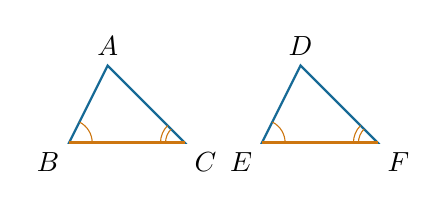
\begin{tikzpicture}[scale=.49]\foreach \shift/\A/\B/\C in {0/A/B/C,5/D/E/F}{\begin{scope}[xshift=\shift cm]\draw[blue,thick](0,0)--(3,0)--(1,2)--cycle;\draw[gold,very thick](0,0)--(3,0);\draw[gold](.6,0)arc(0:63:.6);\draw[gold](2.5,0)arc(180:135:.5);\draw[gold](2.37,0)arc(180:135:.63);\node[above]at(1,2){$\A$};\node[below left]at(0,0){$\B$};\node[below right]at(3,0){$\C$};\end{scope}}\end{tikzpicture}}{Jei vieno trikampio kraštinė ir \textbf{du kampai prie jos} yra atitinkamai lygūs kito trikampio kraštinei ir dviem kampams prie jos, tai trikampiai lygūs. Pavyzdys: $\angle ABC=\angle DEF$, $BC=EF$, $\angle BCA=\angle EFD$.}
\note{\textbf{Atkreipk dėmesį.} Taikydami požymį pagal kraštinę ir du kampus prie jos, įsitikinkime, kad abiejų nurodytų kampų viršūnės yra tos kraštinės galuose.}
\note{\textbf{Kaip įvardyti požymį?} Mokiniai dažnai sako „pagal du kampus ir kraštinę tarp jų“. Vartokime įprastą požymio formuluotę: \textbf{pagal kraštinę ir du kampus prie jos}. Taip aiškiai nurodome, kad abiejų kampų viršūnės yra pasirinktos kraštinės galuose.}
\end{document}
